\chapter{Foundations and Related Work\label{cha:chapter2}}
This section formally discusses the state of the art machine learning techniques and strategies that have been used practically for chatbots.
\\~\\
Chatbots are meant to communicate like humans without being recognized as a machine. Technological elevation using machine learning(ML) and artificial intelligence(AI) have helped a lot in making machines to perform like humans irrespective of complexity of a task. Where increasing trend of ML and AI are providing ease to make an agent learn and communicate autonomously as humans do, meanwhile, there are emerging challenges and problems hindering the pace of the progress. Many major companies are working to make an ideal agent but still are unable to produce one. But with every new year it is getting more mature and the day is not so far when there will be a robot which can make the humans wonder by communicating even better than the creators. In this chapter, the initial purpose to introduce the chatbots is discussed. Why there occurred a need of these agents? The basic and important chatbot techniques are introduced. In addition to that the work and research accomplished so far under this area has enlightened. Let's start with the chatbots definition and brief historical background.     

\section{Chatbots}
According to Shawar and Atwell \cite{ChatbotsAreTheyReallyUseful} initially chatbots were introduced just for fun purpose, based on very basic techniques by replying to the user for the input provided to them. But now their applications are extended just like their scope. Mostly these artificial agents have covered the entertainment sector, information search and assisting humans in e-commerce and business sector. Current chatbots are mainly working for delivering information about the company or for answering simple questions, in other words just for a quick chat. But when it comes to replicate the human beings it is still one of the biggest challenge in the present. As understanding natural language, grabbing feelings, verbal structure, gestures and body language just like living beings are the main hindrances for a machine to act like a human. \cite{CreatingChatbotsToTalk}   
\\~\\
Many companies claim for operating their own chatbots and doing research on them. As mentioned on the website "botnerds.com"\cite{botnerds}, the stats for spring 2017 are as follows:
\begin{itemize}
\item Facebook allege over 100,000 bots on Messenger.
\item Twitter claims approximately 48 million bot accounts.
\item Kik confesses 20,000 bots on its platform.
\item Microsoft Bot Framework declares “minimum 20,000 developers have hired for it.”
\item Wit.ai claims 21,500 workers for development.
\item Small amount of skype bots are also available.
\end{itemize}
Moreover, these bots can be classified according to their serving purpose.

\subsection{Types of Chatbots}
The purpose of serving matters for chatbots in order to be judged as good or bad. 

\subsubsection*{Good Chatbots}
These chatbots lie under the category of agents used for informative purpose or social welfare. As follows \cite{botnerds}:
\begin{itemize}
\item Chat bots.
\item Crawlers.
\item Transactional bots.
\item Informational bots.
\item Entertainment bots: Art bots, Game bots.
\end{itemize}

\subsubsection*{Bad Chatbots}
These are the bots having negative aspects and used for bogus purposes. Some are mentioned below\cite{botnerds}:
\begin{itemize}
\item Hackers.
\item Spammers.
\item Scrapers.
\item Impersonators. 
\end{itemize}
Furthermore, if you dig deep in to it you can figure out precisely the serving purpose of the bots which can be either political, representation i.e. mebots, searching, chatting, working e.g. slack bots used in many work places and voice communication. And some of the well known artificial agents like Alexa, Google Assistant, Siri and Cortana are being used to serve these purposes for a long time \cite{listeningtobots}. Moreover, we can categorize the conversational bots on the basis of functionalities that they are performing.

\subsection{Chatbots Categories}
It is not an easy task to categorize chatbots but according to the market and looking in to the characteristics of the chatbots, they can be classified as mini bots also called "Specialist Bots" and complex bots having ability to perform generally known as "Generalised Bots". \cite{botnerds}
\\~\\
In addition to that specialized bots are mainly the ones that are developed by a developer or small team of developers serving some specific domain. Whereas, generalised bots are those mainly produced by multinational firms and have ability to perform in every aspect and somehow trying to mimic humans in communication.

\begin{figure}[h]
    \centering
    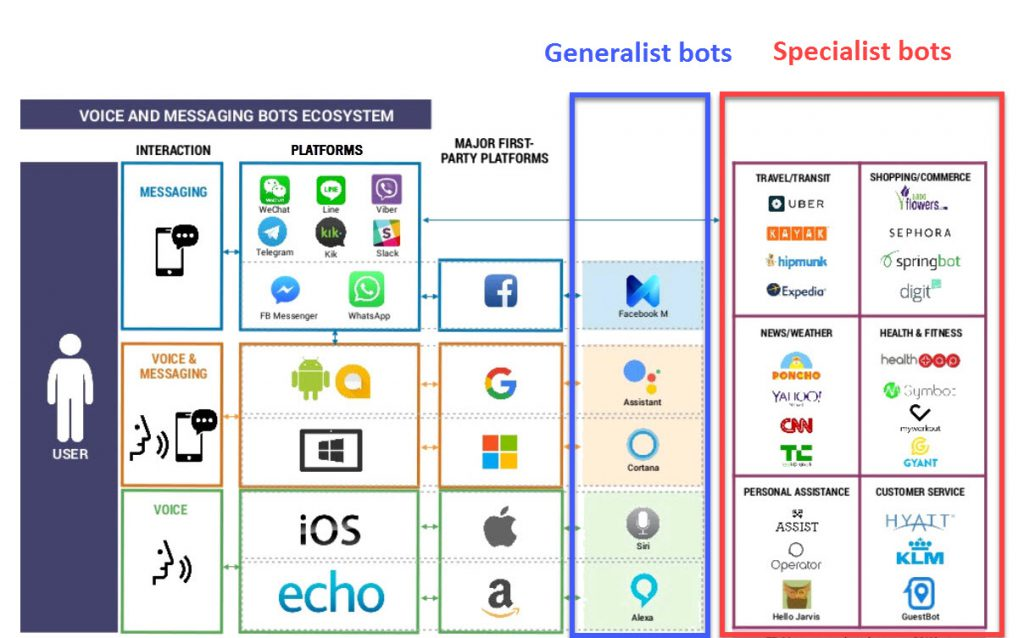
\includegraphics[width=0.9\textwidth]{img/generalist-vs-specialist.jpg}
    \caption{Categorizing Generalized and Specialist Bots \cite{botnerds}}
    \label{fig:ann}
\end{figure}
\\~\\
Now digging in to the generalised bots that how can they be built smart enough to deliver humanly. And then there comes a human characteristic which makes human superior to other beings known as intelligence.

\section{Bots Intelligence}
In order to inject intelligence in to the bots firstly, one should know what is it. So for this reason, a man generated some mathematical models resembling human's brain architecture and tried to train them and made those models to learn by providing some sample information or data. For making the bots intelligent one has to use these models. All existing smart bots use machine learning(ML) and artificial intelligence(AI) techniques to comprehend the language, complex task processing and to figure out the best response. \cite{botnerds}
\\~\\
On basis of the intelligence, bots can be segregated. There are some bots which use and are totally dependent on ML and AI known as "Smart Bots". Those without any AI can be put under the category of "Script Bots" as the just use a script and are totally dumb without it. \cite{botnerds}
\\~\\
Furthermore, AI can also be divided as weak or strong. Weak AI includes pre-defined rules and scopes to make the chatbots work in the right direction. Whereas, strong one is free from such pre-declared rules and is able to learn different behaviours on its own. \cite{CreatingChatbotsToTalk}
\\~\\
Next section explains the high level representation of a conversational agent. 

\section{Chatbots Overview}
Concertedly, there are multiple components that combine to build a chatbot. Whenever there comes any message from the user, it directly passes to language identification module. It varies from simple tag retrieval to more elaborate statistical methods like n-gram models \cite{ngram}. The new message along with the language and potential previous conversation messages retrieved from database, are then pushed to the intent classifier module which identifies the user's conveyed intent. Eventually, a fitting action or a series of actions is produced using the message’s metadata, identified intent and other relevant information from database. Lastly, the action or a sequence is passed to the action handler module as an input and after its execution it generates an appropriate response. \cite{designandimplementation} 
\\~\\
Its diagrammatic overview has been displayed in the Figure \ref{fig:chatbotDiagOverv} below.
\begin{figure}[h]
    \centering
    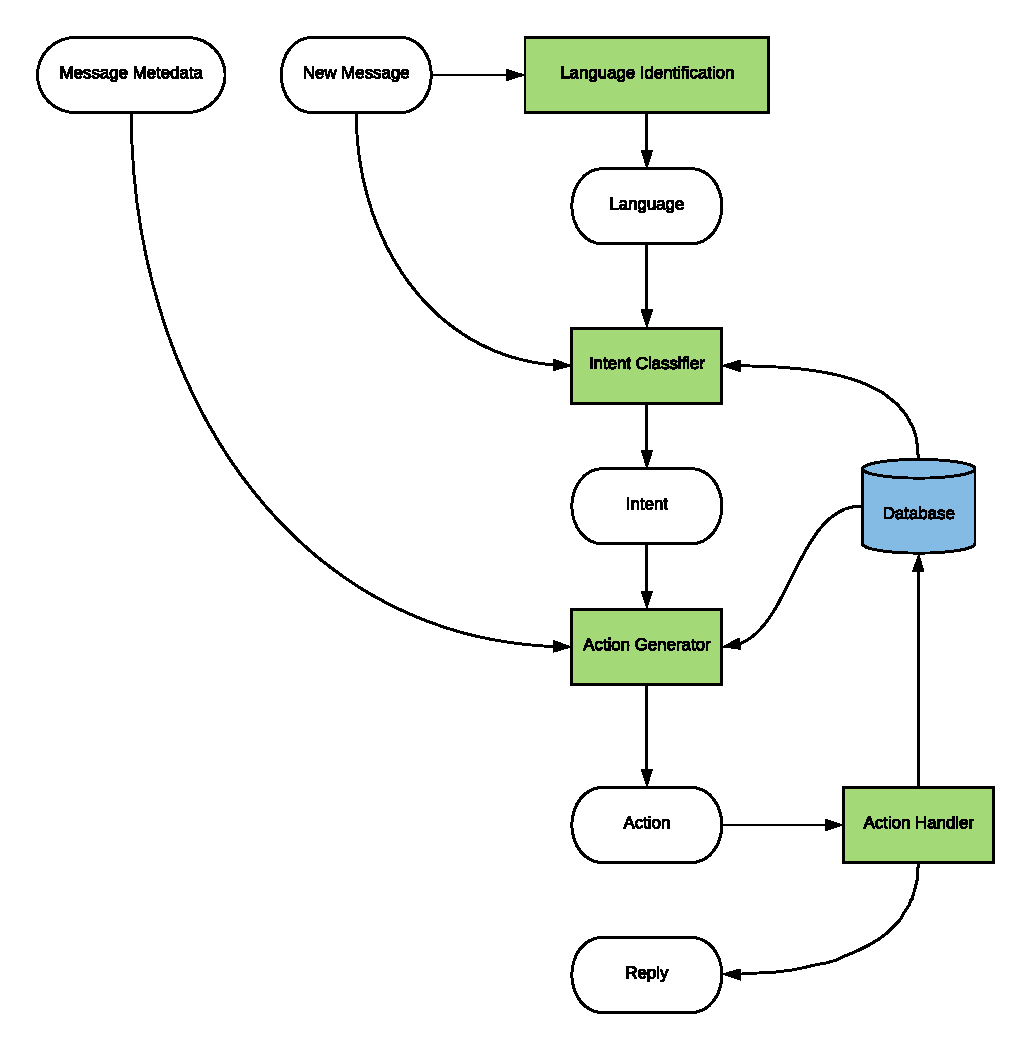
\includegraphics[width=0.9\textwidth]{img/overview.pdf}
    \caption{Chatbots diagrammatic overview \cite{designandimplementation}}
    \label{fig:chatbotDiagOverv}
\end{figure}

\section{Deep Learning Techniques}
In this section some commonly used deep learning will be explained that are used for Natural Language Processing(NLP). When it comes to NLP, Word Embedding and Recurrent Neural Networks are frequently used techniques for deep learning. For Language Identification, it is assumed that utterances can only be written in one language. Furthermore, Intent classification can be done using variety of techniques that vary from Simple Keyword Extraction to Bayesian Inference. Afterwards, response can be generated using retrieval-based and generative-based methods. \cite{designandimplementation}

\subsection{Word Embedding}
Briefly, word embedding technique is used for transforming words in the form of vectors. These mapped vectors can be directly featured in machine learning algorithms. Different methods have already been introduced to exercise this operation. These approaches varies from simple vector count to deep learning methods such as Word2Vec \cite{word2vec}, GloVe \cite{glove} and Skip-gram Model \cite{skipgram}. \cite{designandimplementation}

\subsection{Recurrent Neural Networks}
Recurrent Neural Networks(RNNs) are the neural networks specifically designed for sequenced data. More precisely, such networks work recursively having internal state denoted as \texorpdfstring{C\textsubscript{t}}{C t} at specific time t. Which is passed as an input to the neuron as upcoming time-step and it outputs a value \texorpdfstring{h\textsubscript{t}}{h t} based on \texorpdfstring{C\textsubscript{t}}{C t} at that time-step. But while implementing a simple RNN there comes gradient problems already proven by Pascanu, Mikolov, and Bengio in “Understanding the exploding gradient problem” \cite{gradientproblem}. So to overcome this problem various revised methods have been introduced. According to \cite{designandimplementation} most commonly used ones are mentioned below: 
\begin{itemize}
\item Long Short Term Memory Units \cite{lstm}.
\item Gated Recurrent Units \cite{gru}.
\end{itemize}

\section{Chatbots Tasks and Components}
Chatbots consist of various components and each component is responsible for performing a specific task.

\subsection{Language Identification}
When it comes to larger scale and diversed natural language processing then recognizing a language of a text is a necessary initial step. Some languages contains homographs i.e. Same words with different meanings. It is really a challenging task for an algorithm to understand and grab the correct semantics if language is not known beforehand. \cite{designandimplementation}
\\~\\
It is assumed for this masters thesis that messages will be provided using one language only. Despite of it, there exist methods for inferring different languages in a single document or piece of text and can be found in the document \cite{multilanguagedetection}.

\subsection{Intent Classification}
Another important task that a chatting agent should be able to perform is to classify an intent in the user utterance. It means that a chatbot should be able to detect the purpose of the talk that user is trying to convey. For intent identification, this multi-classification problem is usually solved by labelling the utterances according to the possible user intentions and providing some relative name to them. Furthermore, there exist some techniques to overcome this problem varying from simple keyword extraction to Bayesian inference. These methods are meant to identify the user's request with the help of various messages. Well known LSTM\cite{lstm} networks have been previously used to perform this task due to their high performing and delivering capacity \cite{intentclassificationusinglstm}. \cite{designandimplementation}

\subsection{Knowledge Management}
Knowledge management is directly proportional to intelligence of a chatbot. It means an agent is as much intelligent that how good is it in managing the knowledge provided to it. The task for computers, handling the knowledge progressed significantly in 1980's under the field of "Knowledge Engineering". Methods used for this purpose in the past were consisted of inference tools to shape the facts and evolve new knowledge using first and second order logic. These techniques were used for responding efficiently to ambiguous queries. \cite{designandimplementation}
\\~\\
Knowledge engineering made the functioning easy for conversational bots. As it assists a chatbot to answer a question containing general facts. Apple's Siri and Amazon's Alexa use internal knowledge inference methods to fetch the facts from web and other users resources. \cite{designandimplementation}
\\~\\
In present, Web API calls and optimised requests to the database are extensively used in order to perform this action. Other than that impressive graph-structured ontologies can be used to enhance its performance. \cite{knowledgebase} \cite{designandimplementation}

\subsection{Response Generation}
A conversational bot should have the ability to generate some meaningful response to make the communication effective. So for this purpose it is necessary for a bot to reply coherently according to the context of conversation. This challenging task is executed by following pair of modules:
\begin{itemize}
\item Module to provoke list of competitive responses.
\item Module to select the most relevant reply based on some weighted value or specific metrics.
\end{itemize}
For this sub-challenge, there comes dialogue systems to rescue.

\section{Dialogue Systems}
The importance of human computer interaction has raised drastically in last few years. It is due to its rising potential towards solving daily life problems especially providing aid in commercial challenges. With the advancement of the big data and machine learning, the self functioning virtual assistant is not a dream any more. Based on the applications of conversation companions, the dialogue systems can be divided in to two main categories i.e. Task Oriented Systems and Non-Task Oriented Systems.

\subsection{Task Oriented Systems}
These systems are designed to accomplish a task in some specific domain. The system interprets a message provided by the user, symbolize it to internal state and processes it according to the state of the dialogue. Lastly the final action is performed on it to produce a response in the form of natural language. \cite{surveyondialogsystems}
\\~\\
Mainly natural language understanding is done using statistical models. On the other hand some systems still use human designed pre-defined rules for slot filling and detecting an intent. Which not only results to more time consumption and makes deployment of such system costly, but also restricts the operational domain for the system. To overcome these challenges, deep learning played an important role. Additionally, for extensive representation of state space in pipeline systems, task oriented end-to-end systems have been introduced. \cite{surveyondialogsystems}

\subsubsection*{Pipeline Methods \label{sec:pipelineMethods}}
As mentioned in \cite{surveyondialogsystems} Task oriented systems consisting of pipeline methods inherit following four major components:
\begin{itemize}
\item Natural Language Understanding(NLU) to perceive the semantics of the user utterance.
\item Dialogue state Tracker to supervise the dialogue history and return the recent dialogue state.
\item Policy Learning to predict the upcoming action on the bases of last dialogue state.
\item Natural Language Generation(NLG) for transforming the respective action to the response represented as natural language.
\end{itemize}
Graphical representation of pipeline methods has shown below in the Figure \ref{fig:to}. 
\begin{figure}[h]
    \centering
    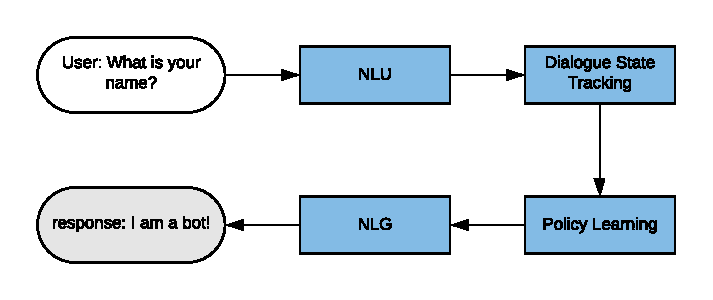
\includegraphics[width=0.9\textwidth]{img/Task_oriented.pdf}
    \caption{Process for Task Oriented Dialog Systems \cite{surveyondialogsystems}}
    \label{fig:to}
\end{figure}
\\~\\
Pipeline based task oriented systems need lot of spoon feeding in particular domain, making them hard to adjust with new domains. In addition to that, the inter-dependency of the components also refrain the system to adapt the new environment. To neglect these challenges end-to-end based task oriented systems have been proposed. \cite{surveyondialogsystems}

\subsubsection*{End-to-End Methods}
Unlike pipeline system, end-to-end system consists of a single module and collaborates with large structured databases. These methods lie under the domain of neural generative models which are discussed below in the section of non-task oriented systems. Many practices have already been made to design a framework for task oriented dialog systems having end-to-end specifications using end-to-end neural generative methodologies. \cite{surveyondialogsystems}

\subsection{Non-Task Oriented Systems}
Main goal of such a system is to communicate with the humans on any topic without restricting it to some specific domain, making them more independent and self sustainable. Applications of such system are entertainment or general conversation with meaningful responses \cite{surveyondialogsystems}.

\subsubsection*{Retrieval-based Methods}
These methods consist of a humongous database containing successive responses. These responses are compared with the information provided by user in form of a message in order to find the best answer for end user. The information provided can usually be a regular expression searching for a specific structures of sentences or any output from machine learning algorithm. This approach benefits the developers by providing a complete control over the responses to prevent any improper answer. \cite{designandimplementation} 
\begin{figure}[h]
    \centering
    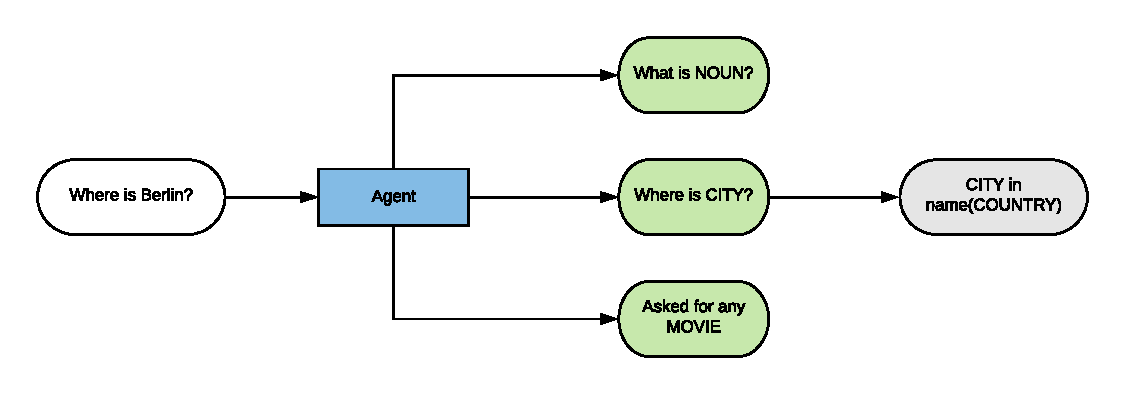
\includegraphics[width=0.9\textwidth]{img/Retrieval_based.pdf}
    \caption{Retrieval-based Methods Example \cite{designandimplementation}}
    \label{fig:rbm}
\end{figure}
\\~\\
The primary and fundamental step to achieve the retrieval-based method is message and response matching. The basic purpose of matching algorithms is to minimize the semantics difference between the responses and the messages. \cite{surveyondialogsystems}

\paragraph*{Single Turn Response Matching}
In this type of matching the only responsible factor for response generation is the message itself. Message context and successive answer are represented as a vector. \cite{surveyondialogsystems}

\paragraph*{Multi Turn Response Matching}
Unlike single turn matching, current utterance along with all past messages are responsible for producing the most suitable response that best matches the overall context of the conversation. \cite{surveyondialogsystems}

\subsubsection*{Generative-based Methods}
Unlike retrieval-based methods, generative-based methods don't need a large database to store pre-generated responses. They are capable of producing a new response based on the user's utterance using generative models. For generating a suitable response it is necessary for the model to be trained enough. Unfortunately, performance of these models is still not sufficient enough to attract the companies due to various restrictions forced by the corporate. \cite{designandimplementation} 

\begin{figure}[h]
    \centering
    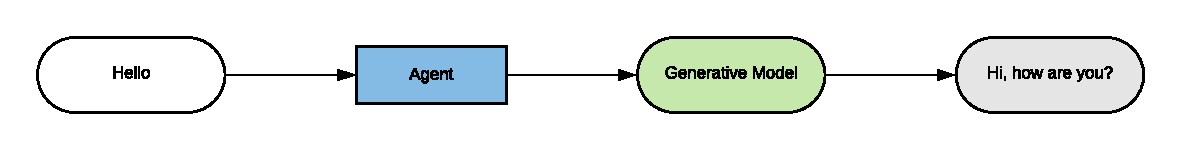
\includegraphics[width=0.9\textwidth]{img/Generative_based.pdf}
    \caption{Generative-based Methods Example \cite{designandimplementation}}
    \label{fig:ann}
\end{figure}
\\~\\
Next section will cover the basis of neural generative models i.e. sequence-to-sequence models. After that there will be explained some research topics underlying these models. 
% \cite{surveyondialogsystems}

\paragraph*{Sequence-to-Sequence Models}
Neural networks are being used by these models in order to symbolize dialog history and to produce useful responses. The systems based on these models doesn't need much knowledge base and pre-defined rules to generate natural language responses. \cite{surveyondialogsystems}

\paragraph*{Dialogue Context}
To keep track of the current state of chatbot and and recent conversation, it is compulsory to take care of the dialogue history and recent user utterances. It helps in understanding the context of dialogues in order to generate appropriate response. Recurrent Neural Networks(RNN) are mainly used for this purpose. \cite{surveyondialogsystems}

\paragraph*{Response Diversity}
To handle response diversity is a challenging task in the systems based on sequence-to-sequence models. As they can provide irrelevant, balanced or completely related answers having some meaning. Inverse Document Frequency(IDF) is mainly used for this purpose. \cite{surveyondialogsystems}

\paragraph*{Topic and Personality}
Topic and personality of the dialogues is another factor to enhance their diversity. By acquiring the fundamental characteristics of dialogues, diversity can be increased and also it leads to gain consistency. \cite{surveyondialogsystems} 

\paragraph*{Knowledge Base}
For making the virtual assistant to perform as humans do there is an essential need of a knowledge base. Not only using outside knowledge base we can cut the informational difference between machines and humans, but can also plant sensibility to artificial conversational agents. \cite{surveyondialogsystems} 

\paragraph*{Interactive Learning}
Eventually the main objective of a dialog system is to be smart enough to do self learning while having an interaction with a user.

\paragraph*{Evaluation}
At the end, the final step is to assess the provoked response quality generated using response generators. Task oriented dialogue systems can be graded using handcrafted methods like rating from the user. Whereas, for non-task oriented dialogue systems its a bit challenging task to evaluate them. METEOR, BLEU and ROGUE are some word overlap metrics to weigh the produced response quality. \cite{surveyondialogsystems}    

\subsubsection*{Hybrid Methods}
Hybrid approaches by combining both above mentioned methodologies have recently been introduced. If response generation fails using retrieval-based methods then it should be produced using generative-based methods. Retrieval based systems gives more accurate results but that could be slow and vague \cite{surveyondialogsystems}. Whereas, neural generative systems have the ability to respond rapidly with the chance of giving useless results \cite{surveyondialogsystems}. So by unifying both of these methods the performance can be enhanced significantly. More study about these methods can be found in \cite{generateifnotretrieve}.

\section{Chatbot Comparison Framework}
On the basis of currently introduced chatbots like Hubot, J.A.R.V.I.S., Pandorabots, Wit.ai etc. the fundamental features vary and can be compared for virtual agents. The key elements are discussed below.

\subsection{Types}
According to \cite{frameworkforunderstandingchatbots} chatting assistants can differ on the basis of their tasks that the are performing. Alertbot is a chatbot that is being used for auto-generating notification for some event occurred. Whereas J.A.R.V.I.S. is a well-known framework for developing artificially intelligent virtual assistants that are capable of rapid self learning and can execute engineering task without any human help. Referring to \cite{softwarebots} chatbot types can be classified as following: 

\subsubsection*{Informative}
Such type of conversational agents are designed to help creators by grabbing required information for some specific task. For example, to produce an alert message for any bug in a program written by some developer. 
% \cite{frameworkforunderstandingchatbots}

\subsubsection*{Collaborative}
These kind of chatbots assist the developers to collaborate and communicate efficiently in order to be more productive. As an example, the collaborative chatbot will alert a developer working on some project, of a chat that is started by some other developers if it involves the one who is working on it and is important for him to be notified. 
% \cite{frameworkforunderstandingchatbots}

\subsubsection*{Automated}
Such chatbots work alongside with the developers to provide aid in tasks accomplishment, having dependencies in one or more projects by detecting the problem caused due to some alteration in a feature. E.g. Auto-generated documentation.
% \cite{frameworkforunderstandingchatbots}

\subsection{Direction}
As mentioned earlier, chatbots differ in the tasks objectives they are performing. On the other hand they function uni-directionally rather than taking the whole conversation in to account. \cite{frameworkforunderstandingchatbots}

\subsubsection*{Input}
Such conversational bots search for some specific keywords or tags pushed by the creator in conversation and fire specific responses based on that keywords or phrases. They are also known as silent bots as they perform their tasks quietly. \cite{frameworkforunderstandingchatbots}

\subsubsection*{Output}
Output chatbots are opposite to input ones. They just need general content or an action to make them operational unlike input bots which require some special keywords to make them trigger any output. Such kind of assistants mostly get activated from some external source and notify about events to a different place. \cite{frameworkforunderstandingchatbots}

\subsubsection*{Bidirectional}
Bidirectional conversational agents work in both directions. They are capable of taking an input and generating an appropriate response accordingly. It can vary from activating just a simple response for some action to real communication. \cite{frameworkforunderstandingchatbots}

\subsection{Guidance}
When it comes to complex chatbots, it is really important to make them function autonomously for their sustainability and practicability.

\subsubsection*{Human Mediated}
These kind of chatbots require human mediation in order to function properly. They can't complete any task on their own. They seek for the relevant information or operational directions from the developer due to which they can not cause much destruction. But if they start to do that then it is very easy for a developer to stop them from further functioning. \cite{frameworkforunderstandingchatbots}

\subsubsection*{Autonomous}
Chatbots which have the ability to perform their tasks on their own and contain all the viable knowledge or having the capability of self learning lie under autonomous agents group. The only problem with such bots is that they can be invasive. \cite{frameworkforunderstandingchatbots}

\subsection{Predictability}
Usually, there is a group of developers responsible of designing any virtual assistant for chatting. With the diverse mindsets of developers there comes uniqueness in specifications and functionalities of a bot. So they can be distinguished on the basis of the genre of tasks they are designed to accomplish. As stated in \cite{frameworkforunderstandingchatbots}, underneath are the following genres:

\subsubsection*{Deterministic}
Chatbots with the deterministic approach perform particularly the same action whenever they observe the similar event or scenario. Such communicating agents involve decision tree to make decisions based on the input provided to them. So it is easier to predict the behaviour of such virtual assistants. 
% \cite{frameworkforunderstandingchatbots}

\subsubsection*{Evolving}
As it is clear from the heading's name that these bots have the ability to evolve themselves. Which means they contain learning element and have the ability to gather knowledge from the past experiences and results. According to which they can regulate their actions. Which results to enhance their performance by making them capable of performing such tasks which were not instructed to them by the developer. But the drawbacks of such agents can't be ignored as they can do self learning and can get out of control while conversation. For example, there was a chatbot for natural language multi-issue bargaining developed by Facebook. Eventually, they had to stop it because it started evolving a language which humans were unable to understand \cite{fbshutdownbot}. 
% \cite{frameworkforunderstandingchatbots}

\subsection{Interactivity}
As no one can deny the fact that it is still a long time to make chatbots act like humans. But the necessity of developing human-like chatbots is rising day by day and lot of research is happening to make chatbots interact as humans do. Although advanced chatbots can have the ability to contain more vocabulary and communicate in a much better way. It helps in enhancing the user experience and promoting chatbots effectiveness. \cite{frameworkforunderstandingchatbots}
\\~\\
As claimed by \cite{frameworkforunderstandingchatbots}, there exist several styles in which chatbots interact with users as mentioned below:

\subsubsection*{Dull}
Chatbots with dull interaction style make conversation using common and repetitive vocabulary and chunks of words. They always use the same welcome message to greet the user without any sense to develop the new meaningful phrase with same semantics. 

\subsubsection*{Alternate Vocabulary}
Such virtual agents consist of a container with multiple equivalent phrases for the same user utterance. They randomly choose the response out of a container for the utterance with same semantics. Which makes these bots superior to dull ones. 
% \cite{frameworkforunderstandingchatbots}

\subsubsection*{Relationship Builder}
Such conversational assistants try to build a good relationship with the developer or end user. Terms used by these chatbots differ from formal to casual and vice versa. They are capable of doing continuous communication. While communicating, they can reach a point to crack a joke for humorous purpose in order to improve the bond and fun experience with the user. 
% \cite{frameworkforunderstandingchatbots}

\subsubsection*{Human-like}
These are the most learning chatbots which use the past chat history for its training in order to become intelligent enough for producing appropriate response for the user query.  
% \cite{frameworkforunderstandingchatbots}

\begin{figure}[h]
    \centering
    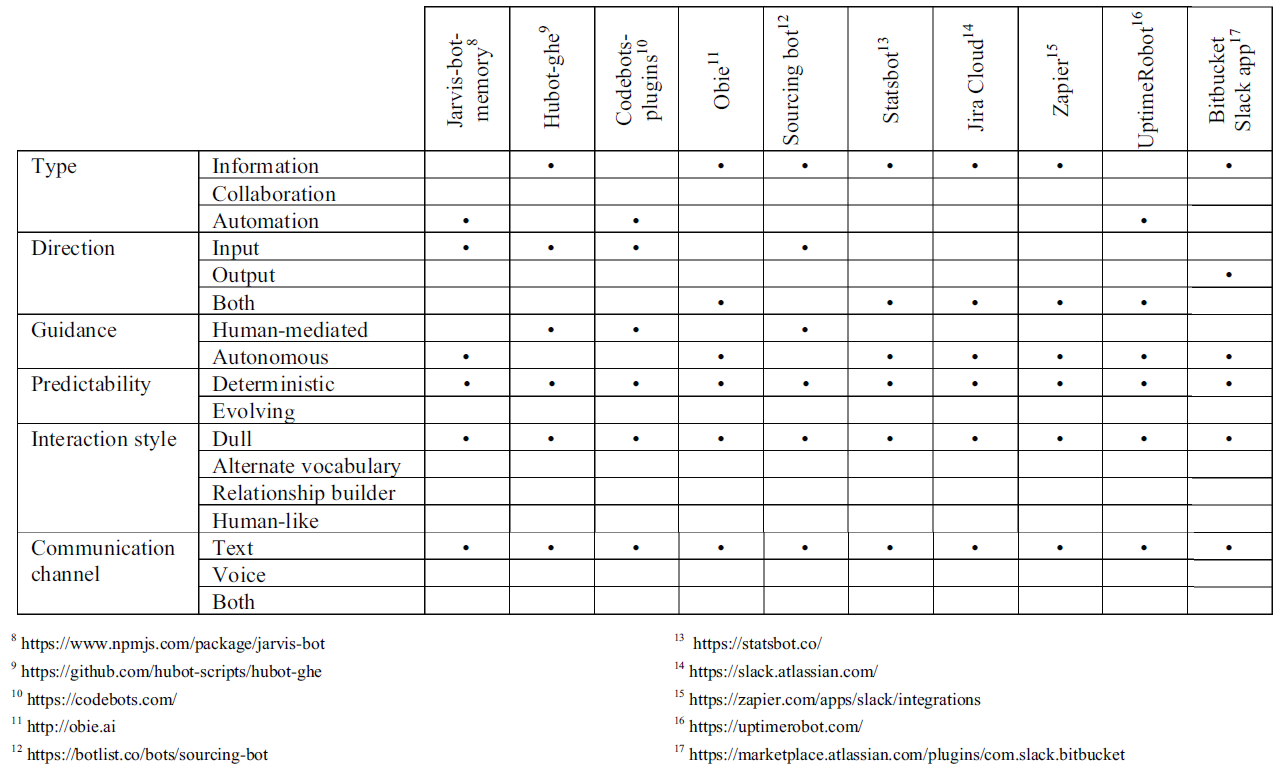
\includegraphics[width=0.9\textwidth]{img/Chatbots_Comparison_Framework.PNG}
    \caption{Comparison framework practiced for software development on selected chatbots. \cite{frameworkforunderstandingchatbots}}
    \label{fig:chatcompfram}
\end{figure}

\subsection{Communication Channel}
There are two types of communication channels that almost all the chatbots are using for communication i.e. messaging platforms for text messages like Slack and speech communication platforms like Alexa. \cite{frameworkforunderstandingchatbots}

\subsubsection*{Text}
These chatbots use text messages for communication. They have an extra advantage as the input and output is in textual form which is easier to understand, store and adapt. It also provides an ease for a developer. \cite{frameworkforunderstandingchatbots}

\subsubsection*{Speech}
Chatbots with voice or speech feature support are more user convenient and provide more realistic and natural mean of communication as they take input using vocals and produce spoken output. Despite of that, they do not implement the facilities which are offered by the ones using text. \cite{frameworkforunderstandingchatbots}

\subsubsection*{Text and Speech}
There also exist such chatbots which have the conversational support using both voice and text channels. They provide the user with an option to configure the way of taking an input and expressing the output. \cite{frameworkforunderstandingchatbots} 

\section{Dialogue Management Systems}
This section covers the role, methods and problems occur while managing dialogue systems. They have been introduced a long time ago under the shadow of systems supporting database queries. One can easily question a computer using natural language or scripted language such as SQL for fetching database information. Dialogue management systems are required for complex utterances from the user in order to deliver decent responses.

\subsection{Role}
Systems designed for dialogue management are meant to imitate conversation processing. Shaping a dialog from any source such as speech, text or any other approach is an essential step for making a dialogue manageable. If there occurs a system failure then communication must not have a full stop. The dialogue manager should be capable of catching a reason of failure and endorsing a dialogue recovery. \cite{dialoguemanagementsystems}

\subsection{Discourse Characteristics}
Conversation or debate between humans is not something that can be easily understandable by computers. It comprises of many complexities. But while having a dialogue between machines and humans, one can make a communication using simpler language but still a person expects that system should hold various features as claimed by \cite{dialoguemanagementsystems} are stated below: 
\begin{itemize}
\item \textbf{General Structure:} Dialogue consists of opening, body and closing. User can handle the dialogue at its opening and closing point. Whereas, management system controls the body part of a dialogue.
\item \textbf{Combined Initiative:} Usually user holds most of the control over a dialogue. Then there comes a system to take over the control for diminishing the misconception, if there occurs any. And this task of management system is mostly gets accomplished by verification of information provided, eliminating the confusion or by restraining the user's reply. 
\item \textbf{Over Gossipy:} It is in a humans nature to provide the extra useful information to others which is not even asked explicitly at that moment. Same goes with dialog management systems that they should be able to do it.
\item \textbf{Contextual Sensation:} System must be capable of sensing and understanding the semantics and context of the dialogue.
\item \textbf{Error Restoration:} If there happens any error or misconception leading to dialog failure then system should be able to restore it and not letting the conversation to stop. 
\end{itemize}

\subsection{Modelling Dialogue Challenges}
Following are some facts and realities of a dialogue stated in \cite{dialoguemanagementsystems}, which can not be ignored and must be taken into account while modelling a dialogue: 
\begin{itemize}
\item \textbf{Turn Switching:} Handling the switching of turns between user and agent or between two agents. 
% \cite{dialoguemanagementsystems}
\item \textbf{Conversational Fillers:} While communicating humans usually use interjections like aah!, nah!, yep! and oops!. Such words are known as fillers as they don't contain any meaning but are useful to increase the cohesiveness and convey the intentions of the user.  
% \cite{dialoguemanagementsystems} 
\item \textbf{Ellipsis:} Ellipsis are words omitted by humans during conversation but can be understood using context of previous discourse. So it is another factor that should be taken under consideration while modelling a dialogue. Otherwise, system will not be able to deliver smartly like humans do. 
% \cite{dialoguemanagementsystems}
\item \textbf{Indirectness:} It involves the communication in which literal meaning of an utterance conveys wrong meaning. But by using the intellectual capabilities, participants can interpret the correct semantics.
% \cite{dialoguemanagementsystems}
\item \textbf{Adjacent Dependency:} It occurs when two participants are communicating and one asks a question but second participant instead of replying to it, posts another related question. Now its a first one turns to respond to the question raised by the second participant in order to get answer of his firstly asked question. 
% \cite{dialoguemanagementsystems}
\item \textbf{Anaphoric and Cataphoric Reference:} Anaphoric reference is used to get the meaning of the recent word by referring to a term used previously in the text. In contrary, cataphoric refers to a word used afterwards in the text to understand the meaning of recently mentioned word. For example, last/next, now/then, I/you etc.
% \cite{dialoguemanagementsystems}
\end{itemize}

\subsection{Dialogue Classification}
Classify the dialogues is not an easy task to perform. Specially when it comes to taxonomize them on the basis of their features. The classification proposed by Dahlbäck in 1995 is based upon the tasks executed by Rubin in 1980 and Clark in 1985. According to them, dialogues can be classified under four dimensions as mentioned in \cite{dialoguemanagementsystems} are:  
\begin{itemize}
\item \textbf{Agent type:} It includes humans and computers with great impact on the language used to communicate. It has been noticed that while having a conversation with virtual agents, humans use utterances conciser, simpler and shorter linguistics.
\item \textbf{Communication Channel:} It underlines many distinguishing  features but the most important one out of them is the method used for communication i.e. spoken or written. Other factors involve transmission styles. 
\item \textbf{Type of Task:} It is another factor having huge impact on the structure of a dialogue. Additionally, task context also have a great affect. Another important aspect having strong impression on dialogue's structure is number of tasks performed by a single dialogue.      
\item \textbf{Mutual Knowledge:} Knowledge shared among the dialogue contestants also has an influence on language which can not be ignored. There exist three ways to deliver the information between dialogue participants.
\begin{enumerate}
    \item Perception between speaker and listener.
    \item Lingual between both.
    \item Cultural knowledge.
\end{enumerate} 
\end{itemize}

\section{Dialogue Management Techniques}
A good dialogue management tool must include two necessary elements concerning interaction between a user and a bot. The first one is referred to as conversation background or history for correctly determining the context of a dialogue. Whereas, second important element is an interaction model designed to govern the system's approach for handling schema of conversation. \cite{dialoguemanagementsystems}
\\~\\
There exist numerous methods to artifact systems for dialogue management. But each system should include some basic components as shown in Figure \ref{fig:gsls}. Input is provided to the system as a text or interpretative speech which is further processed by natural language understanding component to infer the context and semantics. Dialogue manager is mutually connected with all components to deduce all related and meaningful related information, remove confusions and conflicts. Dialog manager's output is being used by response generation unit in order to produce response in the form of natural language or any other suitable representation may be outlined as a text to sense visually. If it is generated as natural language then there comes a speech synthesizer to performs its task by reading it out loud for the user. \cite{dialoguemanagementsystems} 
\begin{figure}[h]
    \centering
    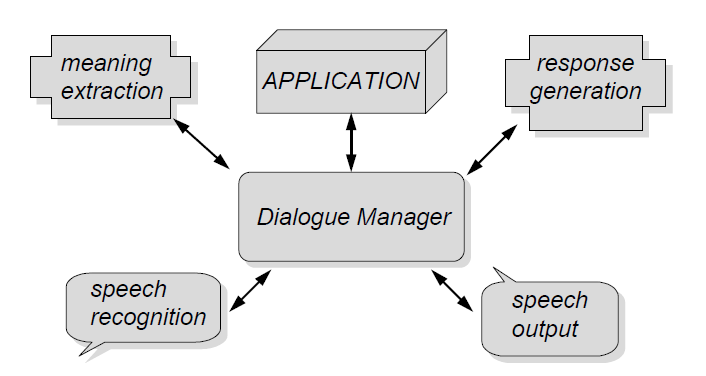
\includegraphics[width=0.9\textwidth]{img/Generic_Spoken_Language_System.PNG}
    \caption{Generic Spoken Language Systems \cite{dialoguemanagementsystems}}
    \label{fig:gsls}
\end{figure}
\\~\\
As Figure \ref{fig:gsls} depicts just an overview of spoken dialogue systems. For more illustrative and detailed demonstration of different units along with the tasks that they are responsible for, just have a look at Figure \ref{fig:dsdm} below.
\begin{figure}[h]
    \centering
    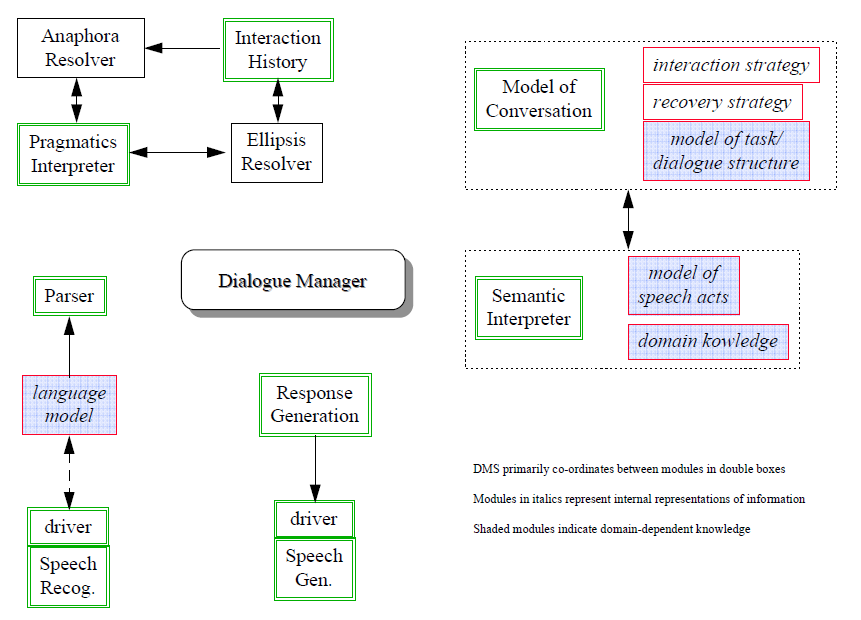
\includegraphics[width=0.9\textwidth]{img/Detailed_Spoken_Dialogue_Manager.PNG}
    \caption{Detailed Spoken Dialogue Manager along with Key Components \cite{dialoguemanagementsystems}}
    \label{fig:dsdm}
\end{figure}

\subsection{Grammars for Dialogue} 
It is the most common initial method out of all the firstly introduced methods. It uses directed grammar from sequential sentences for dialogue description. Usually the grammar describes the architecture of whole communication. According to \cite{dialoguemanagementsystems}, following is the most commonly used approach for this purpose. 
% \cite{dialoguemanagementsystems}

\subsubsection*{Finite State Machines and Graphs}
Finite state models and graphical representations are the simplest methods used for managing a dialogue. Best scenario to get full benefit out of these is, when the structure of the dialogue resembles the structure of the task. Interlinked nodes join to build a graph which minimizes the user choice for selections at that very moment. And with each leading response, the state changes to another node. Like other techniques, it also has advantages along with some disadvantages. As a positive stance, the system has the overall control over the communication by limiting the user choices. On the other hand they also lack the flexibility  to be adapted by some different task and domain. \cite{dialoguemanagementsystems} 
\\~\\
To overcome the flexibility issue, there comes plan based approaches to rescue.

\subsection{Plan-based Methods}
When it comes to complexity, these methods are considered to be more complex for dialogue designing as compared to dialogue grammars approaches. These methods are goal specific like humans as they communicate to achieve different objectives. These methods are used to architect these goals and sub-goals for a task or dialogue. \cite{dialoguemanagementsystems}
\\~\\
Stated below is an application of a plan-based method taken from \cite{dialoguemanagementsystems}.

\subsubsection*{Conversational Games Theory}
It is a well known pattern to develop a dialogue architecture at mass level. In addition to that, it can also be beneficial to design a task oriented dialogue among humans and a computer.  Both grammars from the dialogue and pattern-based approaches are involved in its development. There exists a set of rules or we can call them turns for each game. Which includes the response for some question. So hypothetically, there exists dialogues and each dialogue is responsible to complete some small task. Which collectively results in accomplishment of the main task. And each dialogue is responsible for performing some transactions which represents a sub-task. Whereas, every transaction represents a game associated to some conversation. 
% \cite{dialoguemanagementsystems}

\subsection{Collaborative Methods}
Humans collaborate with each other in order to develop some understanding among them. The main idea behind these methods is to involve both of the participants for a dialogue to get the sense of mutual understanding. Collaborative techniques have main focus on the incentive of the dialogue unlike, pattern-based approaches with having task structure as a main target. Additionally, these methods also try to grasp the dialogue structure. Which means these approaches have the ability for catching general dialogue properties. \cite{dialoguemanagementsystems}

\section{Dialogue Management Systems: Challenges}
There exist two major concerns for a dialogue management system. First one includes the coding strategy for design and structure of a system. Secondly, the recovery technique in order to overcome a particular error is also a challenging task.

\subsection{Coding Strategies}
Strategies used for coding purpose are most often independent of a dialogue structure. They are usually used to design conversation using deterministic approach i.e. finite state machine, or non-deterministic approach i.e. statistical model. Coding scheme and modelling strategy are responsible for the amount of information that can be delivered using a dialogue. There are different types of techniques that can be useful under different circumstances. But the basic need is to understand the user point of view from the utterance which in fact is a challenging task. And for better understanding of a user intention, support can be taken from the context. So for this purpose, a linguistic philosopher Austin in 1962 initiated the research which was later named as Speech Acts Theory after the contributions by Searle in 1969. \cite{dialoguemanagementsystems}  

\subsubsection*{Speech Acts}
Austin initiated it after noticing that some user utterances are not only the statements but can be an order to perform some action. He demonstrated following two sentences to make it more understandable:
\begin{enumerate}
    \item “I bet you six pence it will rain tomorrow”
    \item “I name this ship the Queen Elizabeth”
\end{enumerate} 
These statements can not only be judged as true or false. So he classified such statements as Performative Statements. Whereas, those statements that can be examined using true/false flags were named as Constative Statements.
\\~\\
Later, the classification proposed by Austin was proven wrong. As both types mentioned before can be put under the shadow of illocutionary acts. Illocutionary reflects the true purpose of the statement that can be an offering, promise or a warning. This illocutionary act was named as "Speech Act". Which demonstrates the true view point of the user utterance. 
\\~\\
With its applications, a problem was raised when identified act doesn't match intended user act. To overcome the problem, the identification of perlocutionary act is important. For example, "It is cold in here" seems not to be a statement but a request to turn on the heat or any other related appeal. So, Searle in 1975 declared it as another type of speech act Indirect Speech Act(ISA). But it made the automatic labelling a real problematic task due to the uncertainty of the utterance that if it should be considered literal or interpreted. 
\\~\\
Furthermore, Brown and Yule in 1983, proposed another problem with speech acts while applying them to user utterances. Speech acts need one-to-one mapping between user utterance and an act. But there can be a scenario where multiple user utterances are responsible to complete a speech act or multiple speech acts can be performed with the help of a single utterance.
\\~\\
Considering above mentioned problems with speech acts, Bunt in 1989 came up with another approach to succeed speech acts and that was Dialogue Interpretation Theory(DIT). According to this theory, the dialogues can be classified under two categories: task oriented for controlling a dialogue and proposed content integration. \cite{dialoguemanagementsystems}

\subsubsection*{Dialogue Structure}
A dialogue having independent domain can add some structure to a dialogue while getting converted to dependent morphology. But the structure added is limited to the general acts. As mentioned above, conversational game theory adds a dialogue structure on top of speech act.
\\~\\
Another methodology of adding a structure to a dialogue was introduced by Alexandersson in 1996. It takes a collection of dialogues followed by dialogue acts to produce intentional structure for itself. Which means a dialogue is divided in to goals and sub-goals to gain a structure with some hierarchy. This process can be completed using following three steps as stated by \cite{dialoguemanagementsystems}\cite{automaticacquisition}: 
\begin{enumerate}
    \item Acts in a collection are traversed to convert them to domain independent from dependent hierarchy.
    \item Encapsulate dialogue sequences in different classes. Which are responsible for some functionality or representing a dialogue phase.
    \item Auto-production of context-free-grammar using Bayesian Model.
\end{enumerate} 

\subsection{Error Recovery}
There is a high risk of task failure but it should be made sure that a dialogue must go on. It should be highly prioritize that the dialogue manager must be able to catch the error and handle it properly. Which means it should be able to recover from such faulty situations. The bugs can vary from speech recognition to inaccurate semantic analysis of user's utterance. For this purpose, it is necessary for a manager to encounter it correctly and undergoes some appropriate strategy. So, the taken action may differ depending upon the scenario. It must follow recursive pattern to detect errors that occurred while solving the old one. \cite{dialoguemanagementsystems}
\\~\\
While handling speech recognition, mainly following three types of errors are generated as referred by \cite{communicationaldeviation}\cite{pragmaticinterpretation}: 
\begin{itemize}
\item \textbf{Uncertainty:} It occurs when there is low confidence for a speech input.
\item \textbf{Inconsistency:} It refers to misconception or misunderstanding. Which means the input speech holds high confidence value but opposes the former conversation.       
\item \textbf{Ambiguity:} It occurs when system gets confused between more than one high confidence values for a speech input.
\end{itemize} 
\\~\\
Luperfoy proposed the following four steps recovery method in 1996 as stated by \cite{tutoringversustraining}\cite{dialoguemanagementsystems}: 
\begin{itemize}
\item \textbf{Detection:} Error detection is a challenging task and can also be user dependent to inform the system about it.
\item \textbf{Diagnosis:} It includes error classification.       
\item \textbf{Selecting Repair Plan:} It depends upon the diagnosed error class.
\item \textbf{Executing Interactive Plan:} Selected recovery plan should be executed in an interactive manner to fairly deal with the errors produced by the plan executed.
\end{itemize}

\section{Dialogue Management Systems: Evaluation Methods}
Once the dialogue management system(DMS) is developed and ready to be launched, it must be undergone through some evaluation techniques. It never has been an easy task to perform evaluation for the dialogue systems. Usually its complexity depends upon the criteria of what to evaluate and how to evaluate. In addition to that, assessment is also dependent on different features. The ability of a system to auto-recover itself in case of any error is known as robustness. It should be assessed beforehand during implementation of a system. The other essential thing to evaluate is effectiveness of a system that is, how effective, acceptable and friendly a system is for managing a dialogue. For this reason, there are two methods already being introduced i.e. Quantitative and Qualitative Approaches.

\subsection{Qualitative Methods}
It can be inferred from the name that such methods are used to evaluate the quality of a DMS. These methods involve users to get the mission accomplished. So users opinions play major role in order to make assessment decisions for a system. 
\\~\\
For carrying it out, once the users have adopted and utilized a system, they are provided with a questionnaire to fill or an interview can be conducted for them with different questions regarding performance of a system. Which also includes the questions about performance, natural behavior, user friendliness of the system and how well it performed under certain circumstances. It also varies from person to person that some persons respond positively whilst others can provide negative impressions. Even though the system is same based upon different user preferences. So, it is better to make a user well familiar with a system first and then ask him/her to give an opinion.
\\~\\
Some interviews had been conducted by Dybkjaer in 1995 after making the users familiar with a system which can be found in \cite{qualitativeevaluation}.

\subsection{Quantitative Methods}
In order to assess a DMS quantitatively, already two techniques have been introduced so far i.e. black box and glass box. 

\subsubsection*{Black Box Testing}
It is based upon the input and the respective output without caring about the design and other internal structure of a system. It is just an outer level or top level evaluation and can be performed by the end user.

\subsubsection*{Glass Box Testing}
In this type of assessment, system's internal individual components can be evaluated. And for this purpose, it is necessary for a developer to have the data from the past so that the current output of a component can be compared with the previous one. Such comparison can provide one with the information about accuracy of the the DMS. Such testing can't be performed using black box technique as there is no trustful data available for comparing a dialogue. \cite{dialoguemanagementsystems}

\subsection{Cross-systems Comparison}
In addition to above mentioned evaluation techniques, there also exist some other methodologies to evaluate the dialogue management systems such as objective performance evaluation. It is recommended to perform objective evaluation for the dialogue to make its performance comparable with other management systems. Also in present era, there are several state of the art chatbots available like IBM Watson etc. One can also easily evaluate self created DMS by doing comparison after designing same dialogue on any other state of the art virtual assistants.

\subsection{Evaluation Metrics}
Also there are following evaluation metrics used to quantify the performance of a chatbot according to \cite{differentMeasurementsMetrics}:
\begin{itemize}
\item Dialogue efficiency metrics in terms of matching type.
\item Dialogue quality metrics based on response type.
\item Users' satisfaction assessment metrics.
\end{itemize}
\\~\\
Next chapter illustrates the system architecture and overview of the chatbot named as "Frankenbot" along with its capabilities.

